% Rapatrié depuis le doc de travail (onglet Article FR), révision 144.

\section{Résultats}
\label{sec:6}

\subsection{Caractéristiques de la base générée}
\label{sec:6.1}

La base principale est générée sur le réseau ISOMORPH d'origine, dans la représentation par flux, au niveau de tension 75 (section~\ref{sec:3.7}). À ce niveau, la sévérité varie de 0,68 à 1, la durée des perturbations de 8 à 24 jours et le taux de tension de 1,08 à 1,42 ; l'effet nominal des leviers est réduit d'environ un tiers. Les profils gardent les caractéristiques du tableau~\ref{tab:d5}, afin que la politique reste une intervention définie indépendamment du contexte ; seuls leurs seuils de tolérance sont relevés, à 0,98, 0,95 et 0,92, car la performance minimale médiane d'une crise restant proche de 0,87, les seuils nominaux laissaient les profils prudent et tardif presque toujours inactifs. Ce relèvement conserve l'ordre des profils, seul objet de la comparaison.

Cette configuration a été retenue au terme d'un essai préliminaire d'une quarantaine de configurations, sur un critère unique : le contraste entre politiques, sans lequel l'apprentissage causal n'aurait rien à identifier. La représentation par flux isole les mécanismes de capacité et rend les écarts entre politiques directement interprétables ; le rôle des stocks fait l'objet d'une analyse dédiée (section~\ref{sec:6.5}).

La base compte 2 000 scénarios, soit 8 000 versions de crise, et les cinq natures de perturbation y sont représentées de manière équilibrée (tableau~\ref{tab:d11}). La demande de référence, calibrée sur le volume encore livrable pendant l'incident (équation~\eqref{eq:3}), est très faible lorsque la perturbation touche le hub de Nashville ou l'entrepôt d'Atlanta, par lesquels transite tout le flux : elle reflète la criticité du site touché autant que la taille du réseau, d'où son remplacement par la position de la cible dans la base d'apprentissage (section~\ref{sec:5.1}).

\begin{table*}[htbp]
\caption{Caractéristiques de la base principale.}
\label{tab:d11}
\footnotesize
\begin{tabularx}{\textwidth}{@{}LL@{}}
\toprule
\textbf{Caractéristique} & \textbf{Valeur} \\
\midrule
Scénarios ; versions de crise & 2 000 ; 8 000 \\
Répartition des natures & Panne fournisseur 422, fermeture d'un site de stockage 405, pic de demande 395, congestion 390, coupure de lien 388 \\
Durée de la perturbation, médiane [quartiles] & 16 jours [12 ; 20] \\
Sévérité, médiane [quartiles] & 0,91 [0,82 ; 0,95] \\
Part des articles critiques & 0,20 à 0,53 \\
Coefficient de détermination, médiane [quartiles] & 0,88 [0,79 ; 0,93] \\
Coefficient de détermination sur trajectoire lissée, médiane & 0,91 \\
Versions dont la chute est inférieure à 0,03 & 4,2 \% \\
Indicateurs non finis & 0 \\
Corrélation entre IPC et service perdu observé & 0,97 \\
\bottomrule
\end{tabularx}
\end{table*}

L'ajustement est satisfaisant pour l'essentiel de la base : le coefficient de détermination médian atteint 0,88 et aucun indicateur n'est indéfini. Un quart des versions reste sous 0,8, principalement des crises courtes ou à reprise accidentée. L'indicateur de perte cumulée IPC reste néanmoins très fidèle au service effectivement perdu (corrélation de 0,97), ce qui justifie d'en faire l'indicateur principal de résilience : il dépend peu des imperfections de forme de la courbe ajustée.

\subsection{Effet des perturbations et des profils de gestion sur la résilience}
\label{sec:6.2}

Le tableau~\ref{tab:d12} compare les quatre versions de chaque crise ; les écarts y sont attribuables à la seule gestion (section~\ref{sec:3.6}).

\begin{table*}[htbp]
\caption{Réaction et résilience selon la politique de gestion (2 000 crises).}
\label{tab:d12}
\footnotesize
\begin{tabularx}{\textwidth}{@{}LLLLL@{}}
\toprule
\textbf{Indicateur} & \textbf{Sans réaction} & \textbf{Réactif} & \textbf{Prudent} & \textbf{Tardif} \\
\midrule
Versions avec au moins un levier engagé & sans objet & 98 \% & 88 \% & 56 \% \\
Leviers engagés en moyenne & 0 & 2,8 & 2,0 & 0,7 \\
Détection, jours après le début (médiane) & sans objet & 0 & 1 & 3 \\
Performance minimale (médiane) & 0,87 & 0,89 & 0,88 & 0,87 \\
Retour à la normale, jours après le début (médiane) & 14 & 4 & 11 & 13 \\
IPC, médiane [quartiles] & 0,67 [0,43 ; 1,02] & 0,11 [0,07 ; 0,18] & 0,51 [0,36 ; 0,69] & 0,58 [0,43 ; 0,74] \\
Service perdu, en jours de demande (médiane) & 1,34 & 0,37 & 1,09 & 1,25 \\
Part du service perdu évitée, sur l'ensemble des crises & référence & 73 \% & 18 \% & 14 \% \\
\bottomrule
\end{tabularx}
\end{table*}

Trois constats s'en dégagent. Le premier est la domination de la réactivité. Le profil réactif réduit la perte cumulée de 82 \% en médiane par rapport à l'absence de réaction, contre 17 \% pour le profil prudent et 0 \% pour le profil tardif, dont la moitié des crises ne déclenchent aucune action ; les trois écarts sont significatifs (test des rangs signés de Wilcoxon apparié, p $<$ $10^{-150}$). Dans ce modèle, les leviers n'ont pas de coût et restent engagés jusqu'à la fin de la période observée : agir plus tôt n'a donc jamais d'inconvénient, et cette domination est en partie structurelle (section 7.3).

Le deuxième constat porte sur le mécanisme. La performance minimale est presque identique d'un profil à l'autre, autour de 0,87 : aucune politique n'empêche la chute. La différence tient à sa durée (Fig.~\ref{fig:d5}). Le retour à la normale intervient au quatrième jour pour le profil réactif, contre le quatorzième en l'absence de réaction. La perte cumulée du profil réactif devient ainsi indépendante de la durée du choc (corrélation de rangs de Spearman de 0,01), alors qu'elle en dépend nettement sans réaction (0,48), sous le profil tardif (0,37) et sous le profil prudent (0,25). Dans la plage étudiée, la sévérité pèse peu sur la perte (0,08) : à ce niveau de tension, presque toutes les perturbations sont des ruptures franches, et c'est leur persistance, non leur intensité, qui fait la crise.

\begin{center}
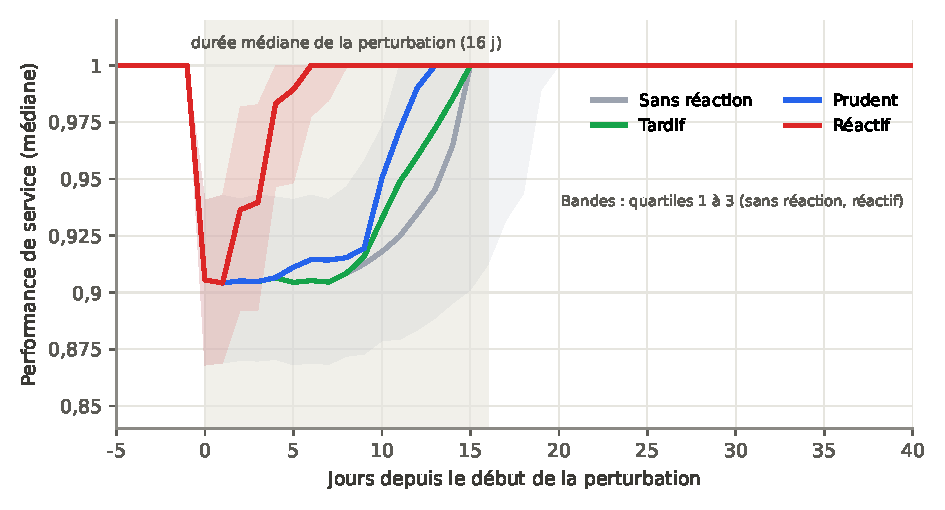
\includegraphics[width=\textwidth]{figures/Fig5_trajectoire_mediane.pdf}
\captionof{figure}{Trajectoire médiane de la performance selon la politique de gestion, sur les 2 000 crises de la base principale, recalées sur le début de la perturbation. Les bandes indiquent l'écart entre premier et troisième quartiles, sans réaction et sous le profil réactif.}\label{fig:d5}
\end{center}

Le troisième constat concerne le choix des leviers : le profil tardif n'engage que des leviers de demande, faute de pouvoir escalader au-delà de ses deux premiers choix pendant la crise, le profil prudent s'appuie surtout sur les stocks et la capacité additionnelle, le profil réactif sur le reroutage et la capacité. Leur efficacité dépend de la nature de la perturbation (tableau~\ref{tab:d13}).

\begin{table*}[htbp]
\caption{Réduction médiane de la perte cumulée par rapport à l'absence de réaction, selon la nature de la perturbation.}
\label{tab:d13}
\footnotesize
\begin{tabularx}{\textwidth}{@{}LLLL@{}}
\toprule
\textbf{Nature} & \textbf{Réactif} & \textbf{Prudent} & \textbf{Tardif} \\
\midrule
Panne fournisseur & 84 \% & 0 \% & 0 \% \\
Coupure de lien & 73 \% & 17 \% & 0 \% \\
Fermeture d'un site de stockage & 82 \% & 10 \% & 2 \% \\
Pic de demande & 87 \% & 23 \% & 13 \% \\
Congestion & 78 \% & 41 \% & 15 \% \\
\bottomrule
\end{tabularx}
\end{table*}

Le profil prudent est sans effet sur une panne fournisseur, que le déstockage ne compense pas, mais réduit de 41~\% la perte d'une congestion, choc diffus que des leviers globaux atténuent ; le profil réactif est le moins efficace face à une coupure de lien, dont les effets se propagent aux voies de secours.

Ces effets dessinent des contextes où une politique moins interventionniste suffit. En classant la perte cumulée en trois niveaux de même effectif, le profil prudent atteint le même niveau que le profil réactif dans 18~\% des crises, et le profil tardif dans 14~\%. Cette proportion atteint 31~\% pour les perturbations de 12 jours au plus, mais tombe à 11~\% au-delà de 18 jours : une crise courte peut être gérée sobrement, une crise longue exige de la réactivité. C'est cette dépendance au contexte que le réseau bayésien doit restituer (section~\ref{sec:6.3}).

Pour vérifier que ces résultats ne tiennent pas à la seule topologie d'ISOMORPH, un lot de contrôle de 500 scénarios a été généré sur le réseau paramétrique avec les mêmes réglages. Les crises y sont moins profondes (performance minimale médiane de 0,91) et l'ajustement moins bon, mais la perte cumulée reste très fidèle au service perdu (corrélation de 0,97). Les grandes proportions sont remarquablement stables : la part du service perdu évitée atteint 67~\%, 17~\% et 13~\% pour les profils réactif, prudent et tardif, contre 73~\%, 18~\% et 14~\% sur ISOMORPH. La topologie modifie en revanche l'efficacité des leviers selon la nature du choc : sur le réseau paramétrique, dont les voies de secours sont de faible capacité, le profil réactif ne réduit plus que de 25~\% la perte d'une coupure de lien et de 53~\% celle d'une fermeture, contre 73~\% et 82~\% sur ISOMORPH. L'effet d'une politique dépend donc conjointement de la nature du choc et de la redondance du réseau.

\subsection{Performance du réseau appris}
\label{sec:6.3}

Le réseau est appris sur 1 600 scénarios, soit 6 400 versions de crise, et évalué sur les 400 restants (section~\ref{sec:5.4}). La structure obtenue (Fig.~\ref{fig:d6}) compte 41 arcs, sans aucun arc contraire à l'ordre des paliers, et retrouve le mécanisme principal de la section~\ref{sec:6.2} : la perte cumulée dépend directement de la politique, de la profondeur $h$ et de la durée $d$ du palier dégradé, et cette durée dépend à son tour de la politique, de la durée de la perturbation et du délai de réaction. La politique agit donc sur la durée de la crise plutôt que sur sa profondeur. La nature de la perturbation conditionne les familles de leviers mobilisées ; la part des articles critiques reste isolée dans la plage étudiée.

\begin{center}
\fbox{\parbox{0.92\textwidth}{\footnotesize [FIGURE À INSÉRER. Source : BayesArtist, apprentissage du fichier \texttt{bayesartist\_apprentissage\_lotA.csv} avec les contraintes \texttt{bayesartist\_contraintes\_isomorph.json} (Greedy Hill Climbing, score BIC, lissage de Laplace), puis « Appliquer au canevas » avec paliers colorés. Contenu attendu : 20 nœuds et 41 arcs, disposés en cinq colonnes de gauche à droite (contexte, politique, réponse, mécanisme, résilience). Pour la lisibilité, mettre en évidence le chemin principal : profil vers $d$ (durée du palier dégradé) et vers IPC ; durée de la perturbation et délai de réaction vers $d$ ; $h$ et $d$ vers IPC. Si la capture reste trop dense, envoyer à Claude le fichier .bif pour une version redessinée.]}}
\captionof{figure}{Réseau bayésien appris sous contraintes, variables colorées par palier de l'ordre temporel d'une crise.}\label{fig:d6}
\end{center}

\begin{table*}[htbp]
\caption{Pronostic de la classe de perte cumulée sur les crises de test.}
\label{tab:d14}
\footnotesize
\begin{tabularx}{\textwidth}{@{}LLL@{}}
\toprule
\textbf{Modèle} & \textbf{Classement correct} & \textbf{Score de Brier} \\
\midrule
Distribution uniforme ou classe majoritaire & 34 \% & 0,667 \\
Politique de gestion seule & 60 \% & 0,494 \\
Réseau appris, contexte et politique & 65 \% & 0,466 \\
\bottomrule
\end{tabularx}
\end{table*}

Le pronostic, établi à partir des seules variables connues au moment de décider, classe correctement 65~\% des crises de test, contre 34~\% pour la classe majoritaire et 60~\% pour un modèle fondé sur la seule politique (tableau~\ref{tab:d14}). Le gain apporté par le contexte est réel mais modeste. La courbe d'apprentissage est presque plate, de 62,5~\% avec 200 scénarios à 63,7~\% avec 1 600 : la taille de la base n'est pas le facteur limitant, c'est l'information disponible au moment de décider. La perte dépend notamment de la tension du réseau, que le générateur n'exporte pas (section~\ref{sec:7.3}).

Le diagnostic est bien calibré pour la politique et la durée. Pour les crises de test à forte perte, la probabilité a posteriori de chaque politique (sans réaction, tardif, prudent, réactif) vaut 0,42, 0,32, 0,26 et 0,01, pour des fréquences observées de 0,41, 0,33, 0,26 et 0,005 ; celle d'une perturbation longue vaut 0,41, comme sa fréquence observée. Il l'est moins pour la nature du choc et la position de la cible : les crises touchant un point de passage obligé, 6~\% de la base, sont trop rares pour que le score retienne leurs effets propres.

La préconisation dépend de l'objectif fixé. Avec l'objectif d'une perte faible, seul le profil réactif l'atteint régulièrement, dans 90 \% des crises de test, et aucune autre politique ne réussit lorsqu'il échoue : la règle préconise alors toujours ce profil. Avec l'objectif moins exigeant d'une perte qui ne soit pas forte, un arbitrage apparaît entre sécurité et sobriété, que règle le seuil $\theta$ (tableau~\ref{tab:d15}). La référence a posteriori montre l'enjeu : dans 67 \% des crises de test, une politique plus sobre que le profil réactif aurait suffi, et dans 42 \% l'absence de réaction elle-même.

\begin{table*}[htbp]
\caption{Préconisation sur les crises de test, objectif d'une perte cumulée non forte.}
\label{tab:d15}
\footnotesize
\begin{tabularx}{\textwidth}{@{}LLL@{}}
\toprule
\textbf{Règle} & \textbf{Objectif atteint} & \textbf{Préconisations plus sobres que le profil réactif} \\
\midrule
Toujours le profil réactif & 99,2 \% & 0 \% \\
Réseau appris, $\theta$ = 0,9 & 99,2 \% & 0 \% \\
Réseau appris, $\theta$ = 0,8 & 97,5 \% & 15 \% \\
Réseau appris, $\theta$ = 0,7 & 86,2 \% & 37 \% \\
Réseau appris, $\theta$ = 0,6 & 69,5 \% & 84 \% \\
Référence a posteriori : politique la plus sobre ayant réussi & 99,2 \% & 67 \% \\
\bottomrule
\end{tabularx}
\end{table*}

Avec $\theta$ = 0,8, le réseau préconise une politique plus sobre dans environ une crise sur sept, pour un taux de réussite de 97,5 \%, soit moins de deux points sous la politique la plus interventionniste. À ce niveau d'exigence, la sobriété repose entièrement sur la durée prévue du choc : lorsque cette information est retirée de la description de la crise, la même règle ne préconise plus aucune politique sobre. Une estimation de la durée d'une perturbation a donc une valeur décisionnelle propre : elle permet d'économiser des leviers sans dégrader la résilience.

\subsection{Étude de cas illustrative}
\label{sec:6.4}

Deux crises de même nature illustrent l'usage du réseau. Dans la première, un site de stockage situé sur un point de passage obligé, comme l'entrepôt d'Atlanta, est fermé pour une longue durée. Le réseau (Fig.~\ref{fig:d7}) donne une probabilité de forte perte de 0,69 sans réaction, de 0,55 sous le profil tardif, de 0,44 sous le profil prudent et de 0,01 sous le profil réactif. Seul ce dernier atteint l'objectif avec une probabilité suffisante : la préconisation est sans ambiguïté, quel que soit le seuil retenu.

Dans la seconde, un site de stockage redondé est fermé pour une courte durée. La probabilité de forte perte tombe à 0,30 sans réaction, 0,22 sous le profil tardif et 0,20 sous le profil prudent. Avec $\theta$ = 0,8, le profil prudent atteint l'objectif avec une probabilité de 0,80 et devient la préconisation : face à un choc bref sur un site doublé, une réaction fondée sur le déstockage suffit, et mobiliser le reroutage et la capacité additionnelle n'apporterait qu'un gain marginal.

\begin{center}
\fbox{\parbox{0.92\textwidth}{\footnotesize [FIGURE À INSÉRER. Source : BayesArtist, réseau appris de la figure~\ref{fig:d6}, mode inférence. Évidences à poser : nature = \texttt{fermeture\_entrepot}, cible = \texttt{passage\_oblige}, duree = fort. Puis fixer successivement profil = none, tardif, prudent, reactif, et capturer la distribution du nœud IPC à chaque fois. Valeurs de contrôle pour la classe « fort » : 0,69, 0,55, 0,44 et 0,01. Présentation conseillée : les quatre captures assemblées côte à côte, ou une seule capture avec le profil réactif et les évidences visibles. Variante : Claude peut produire un diagramme en barres empilées des quatre distributions.]}}
\captionof{figure}{Pronostic de la perte cumulée selon la politique, pour la fermeture longue d'un site situé sur un point de passage obligé.}\label{fig:d7}
\end{center}

Le diagnostic éclaire le cas inverse, celui d'une crise à forte perte gérée par un profil prudent. Le réseau y associe une perturbation longue, avec une probabilité de 0,39 contre 0,33 a priori, un recours au déstockage presque certain (0,95) et une escalade jusqu'à trois leviers ou plus (0,40 contre 0,23 a priori). Il désigne ainsi une crise trop longue pour la politique choisie : le gestionnaire a escaladé, mais à partir de leviers de stock dont l'effet s'épuise, sans atteindre à temps le reroutage. Ce diagnostic oriente l'action corrective vers la politique, plus réactive ou dotée d'un autre ordre de leviers, plutôt que vers le réseau.

\subsection{Sensibilité à la couverture de stock}
\label{sec:6.5}

La représentation temporelle permet d'étudier le rôle des stocks, que la base principale neutralise. Sur le réseau ISOMORPH, avec ses délais de trajet d'origine, 60 crises ont été simulées pour chaque nature de perturbation et chaque couverture, sans réaction du gestionnaire, et l'on a compté celles qui produisent une baisse de service visible (Fig.~\ref{fig:d8} ; valeurs détaillées au tableau~S4 du matériel supplémentaire). La représentation par flux sert de référence.

\begin{center}
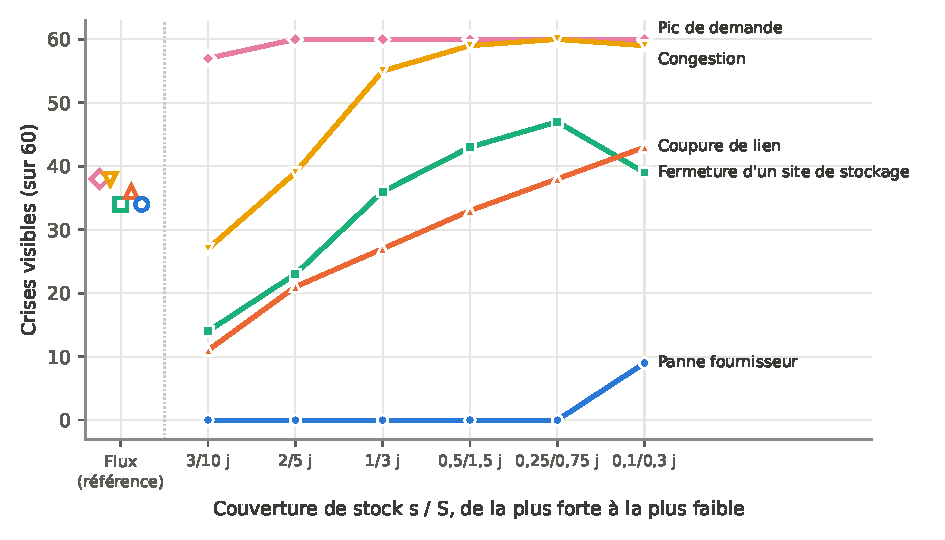
\includegraphics[width=\textwidth]{figures/Fig8_couverture_stock.pdf}
\captionof{figure}{Nombre de crises visibles sur 60 selon la couverture de stock, par nature de perturbation (réseau ISOMORPH, sans réaction). Les symboles creux, à gauche, donnent la référence de la représentation par flux.}\label{fig:d8}
\end{center}

Trois comportements se dégagent. Pour les ruptures de distribution, coupure de lien, fermeture d'un site de stockage et congestion, la couverture agit comme un levier de robustesse progressif : plus elle est faible, plus les crises visibles sont nombreuses, de 11 à 43 sur 60 pour une coupure de lien et de 27 à 59 pour une congestion. La frontière entre robustesse et résilience évoquée en section 4.4 se déplace donc de manière contrôlée avec le niveau de stock. Les pannes fournisseur sont au contraire absorbées dès que la couverture atteint un quart de jour, y compris pour des pannes de 15 à 60 jours à la couverture par défaut : la calibration de la demande borne le manque à servir pendant une panne, que quelques jours de stock suffisent à compenser. Enfin, le pic de demande est mieux absorbé sans stocks qu'avec : dans la représentation par flux, toute marge de capacité sert instantanément le surcroît de demande, alors qu'avec des délais, ce surcroît doit d'abord être prélevé sur des stocks dimensionnés sur le débit nominal, que le recomplètement ne reconstitue qu'après un délai.

La couverture de stock n'est donc pas un levier universel de résilience. Elle protège contre les pertes de capacité de distribution, est presque superflue contre une défaillance amont de faible ampleur, et ne protège pas contre un choc de demande, qui appelle des leviers de capacité ou de demande. Ces résultats, obtenus sans réaction du gestionnaire et à couverture uniforme, n'épuisent pas la question : l'interaction entre couverture et politique de gestion reste à étudier (section 7.3).
